\subsection{Urban Macro Scenario}
\label{subsec:exp2-urban-macro}

The urban macro scenarios is based on the Charles de Gaulle Etoile in Paris, which is a dense urban environment with tall buildings and many obstacles.
The gNB is placed at the top of the Arc de Triomphe at a height of $25$ m and UEs are distributed in a circle of radius $500$ m around the gNB.
The antennas are configured to use the $3.5$ GHz carrier frequency, which is in the sub 6-Hz range.
This scenario is one of the challenging scenario for 6G network deployments due to the high density of buildings and obstacles.

\subsubsection{Application-related Metrics}
\label{subsubsec:exp2-urban-macro-flow}

Figure \ref{fig:exp2-urban-macro-flow} illustrates the application-related metrics for the urban macro scenario, comparing ns-3 (solid bars) and Sionna RT (hatched bars) across various antenna configurations.
Among the traffic types, data-intensive applications such as FTP and video streaming achieve the highest throughput in both simulators.
For FTP, ns-3 outperforms Sionna RT at the $2 \times 2$ configuration where ns-3 achieve roughly $16.8$ Mbps whereas Sionna RT achieve $15.2$ Mbps.
But as the gNB array size increase to $4 \times 4$ and $8 \times 8$, Sionna RT perform better than ns-3 and achieve nearly $19.5$ Mbps whereas ns-3 achieve $18.5$ Mbps.
The statistical ns-3 approach performs well generally but Sionna RT approach performs better at larger array size as it can better leverage massive MIMO spatial multiplexing by capturing multipath components such as reflections and diffractions from the buildings and environment.
In contrast, for video streaming application, ns-3 consistently achieve higher than Sionna RT across all antenna configurations.

For Sionna RT, higher packet loss for video traffic is observed in downlink which values are $9.5\%$, $7.6\%$ and $4.6\%$ respectively for $2 \times 2$, $4 \times 4$ and $8 \times 8$ antenna configurations.
Ns-3 performs better than Sionna RT for video traffic and for FTP traffic under $2 \times 2$ configuration, however, Sionna RT outperforms ns-3 for FTP traffic under $4 \times 4$ and $8 \times 8$ configurations.
Overall, increasing the antenna array size significantly reduce packet loss for most of the applications in both simulators.
In the uplink, the packet loss for all most all of the applications are very high for both simulators, ranging from $15\%$ for VoIP to nearly $100\%$ for gaming and social applications in Sionna RT.
This reflects the impact of harsh environment conditions on the constrained transmission power of UEs which struggles to overcome severe blockages, resulting in poor uplink condition.
Interestingly, Sionna RT still achieve higher throughput than ns-3 for gaming and FTP traffic in uplink eventhough Sionna RT observe higher packet loss than ns-3 for both applications.

Packet delay and jitter metrics further align with these observations.
Downlink delay is worst for video and FTP traffic where Sionna RT achieve $295$ ms, $220$ms, and $175$ ms for FTP and $220$ ms, $145$ ms, and $65$ ms for video, respectively for $2\times2, 4\times4, 8\times8$ antenna configurations.
Ns-3 also observes high delay for video and FTP traffic in downlink as well, however, it is lower than Sionna RT.
The reason Sionna RT experience higher delay is because the detailed multipath components captured by ray-tracing introduce longer propagation paths and varying signal arrival times, increasing the queuing delay.
Jitter remains relatively low in both simulators for all the applications but ns-3 occasionally reports high spike for application like FTP and gaming.

\begin{figure*}[t]
    \centering
    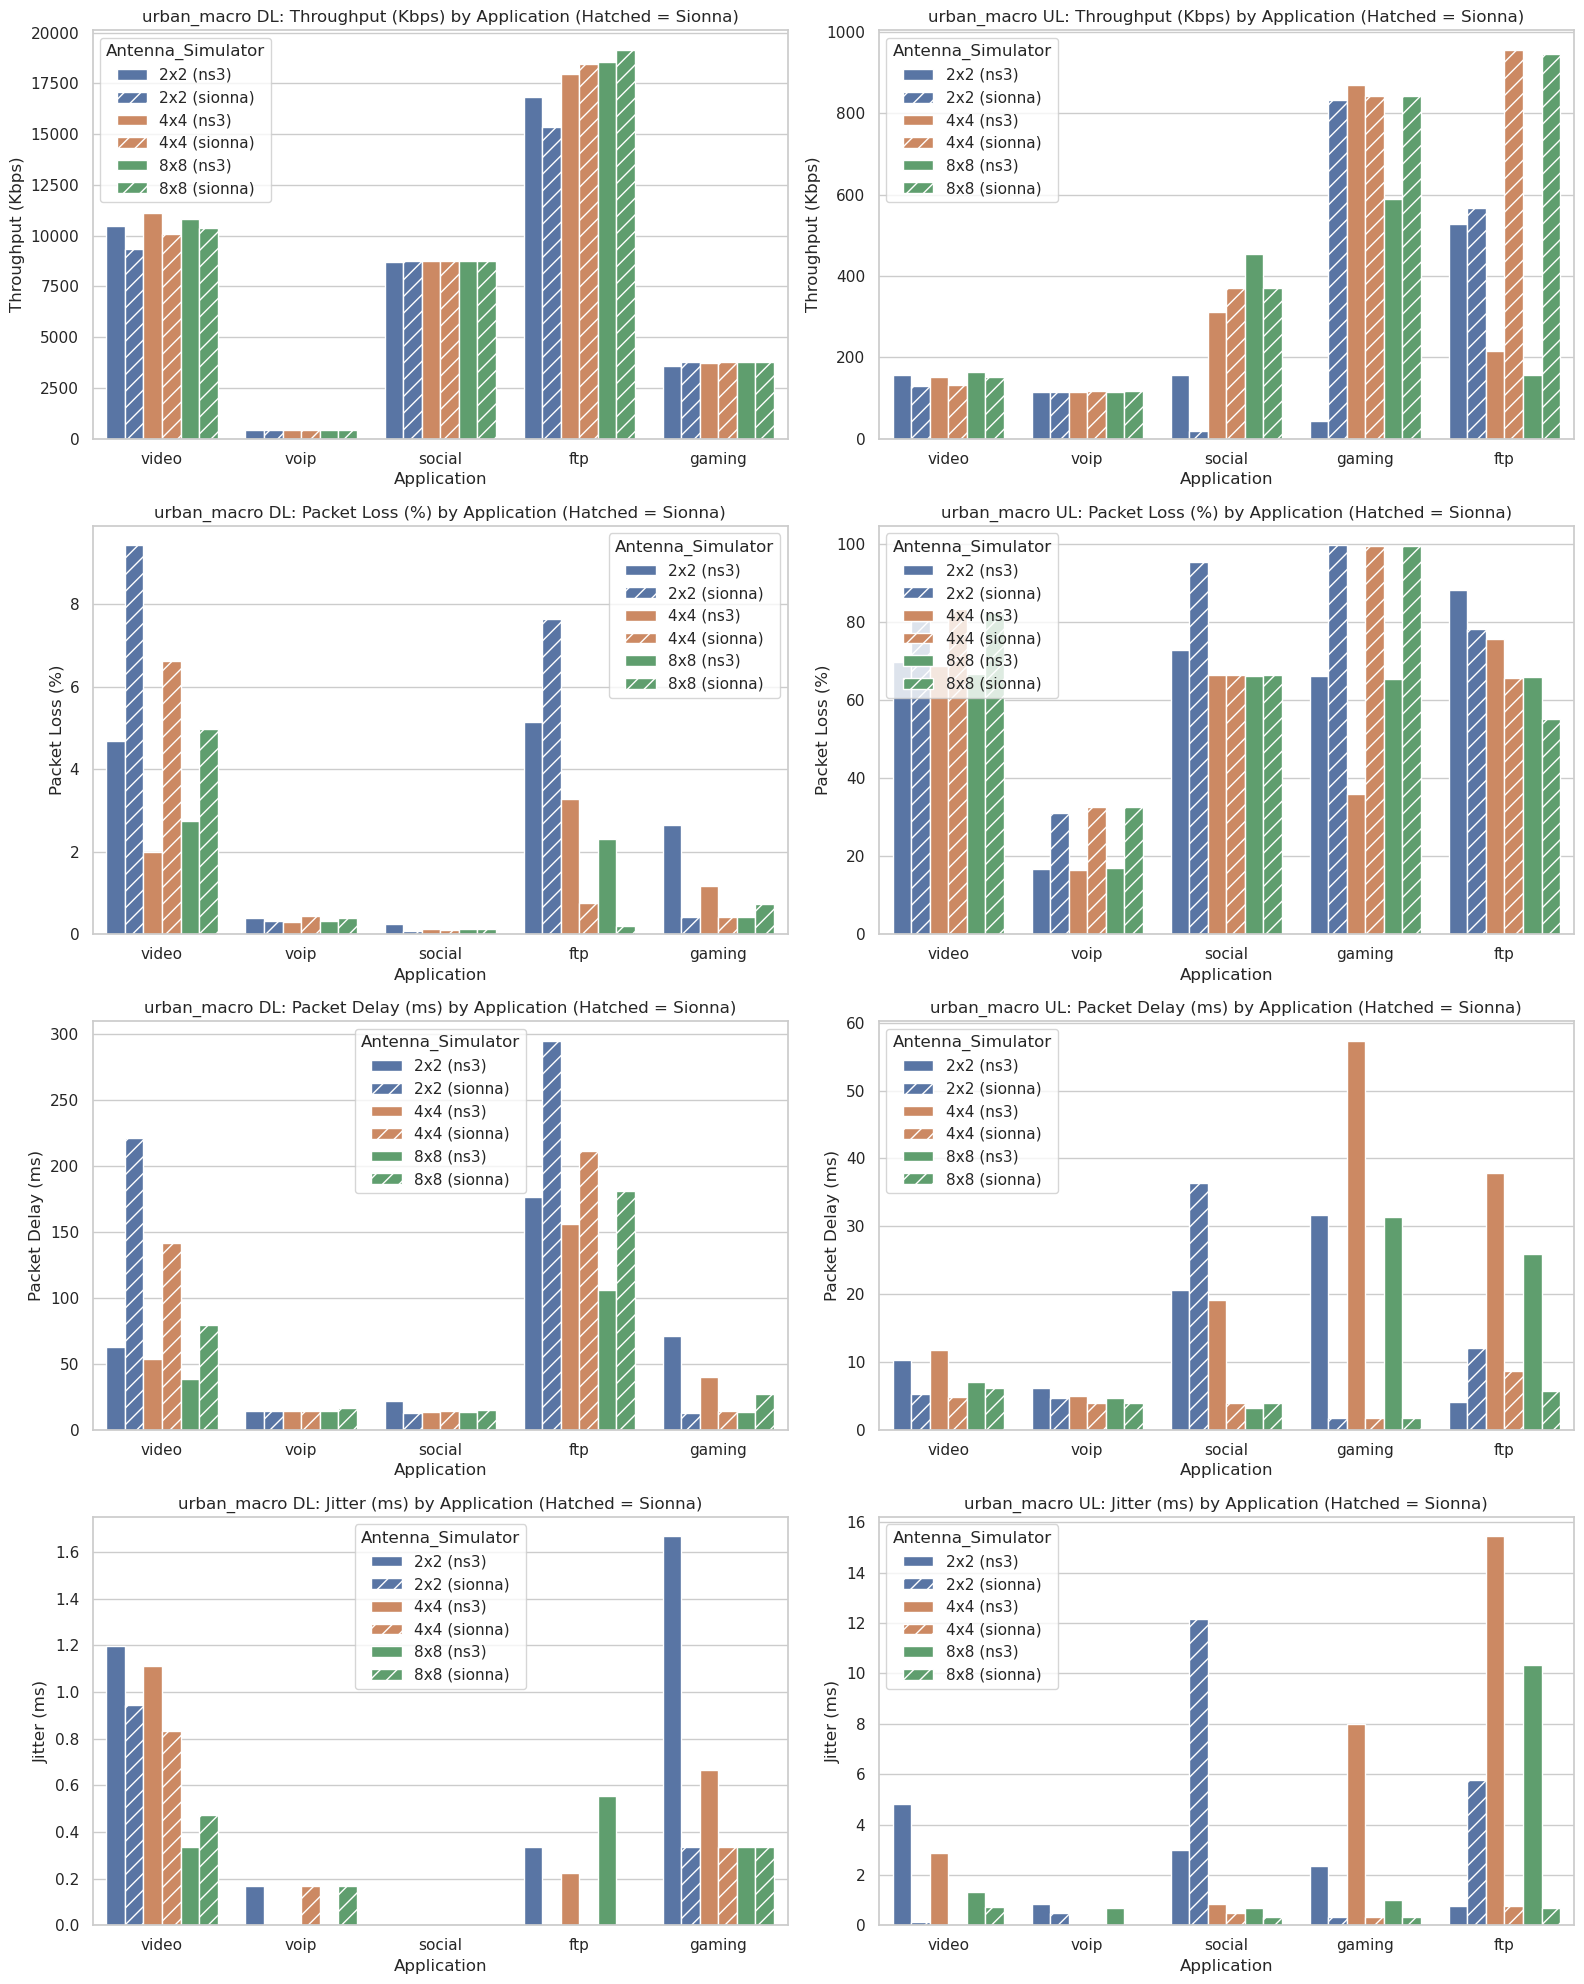
\includegraphics[width=\textwidth]{images/urban_macro_flow_metrics.png}
    \caption{Urban macro Application-related metrics by traffic type, direction, and
        gNB array size.}
    \label{fig:exp2-urban-macro-flow}
\end{figure*}


\subsubsection{Propagation-related Metrics}
\label{subsubsec:exp2-urban-macro-propagation}

The propagation-related results are presented in Figure \ref{fig:exp2-urban-macro-propagation}.
Path loss and received power remain consistent across all antenna size in both simulators at roughly $83.5$ dB and $-37.5$ dBm respectively.
Both ns-3 and Sionna RT achieve nearly identical values for propagation related metrics but differences can only be observed in path delay, CQI and MCS.
Ns-3 estimate a path delay of approximately $220$ ns while Sionna RT estimate higher delay around $360$ ns across all antenna configurations.
Higher delay in Sionna RT was due to taking into consideration for multipath components.

Similarly, lower CQI and MCS values are observed in Sionna RT than ns-3 for all antenna configurations.
For instance, in the $2 \times 2$ configuration, Sionna RT reports an average CQI of $9.5$ and MCS of $16.5$ while ns-3 estimates a CQI of $10.5$ and MCS of $17.5$.
Nevertheless, increasing gNB array size from $2 \times 2$ to $8 \times 8$ improves CQI and MCS in both simulators.
For example,  Sionna RT reports an average CQI of $10$ and MCS of $17$ at $8\times8$ configuration while ns-3 estimates a CQI of $11$ and MCS of $18$.
Improving CQI and MCS according to gNB array size validate that increasing the array size enhances beamforming capabilities and effectively reduces impact of environment and improves overall link quality.


\begin{figure*}[t]
    \centering
    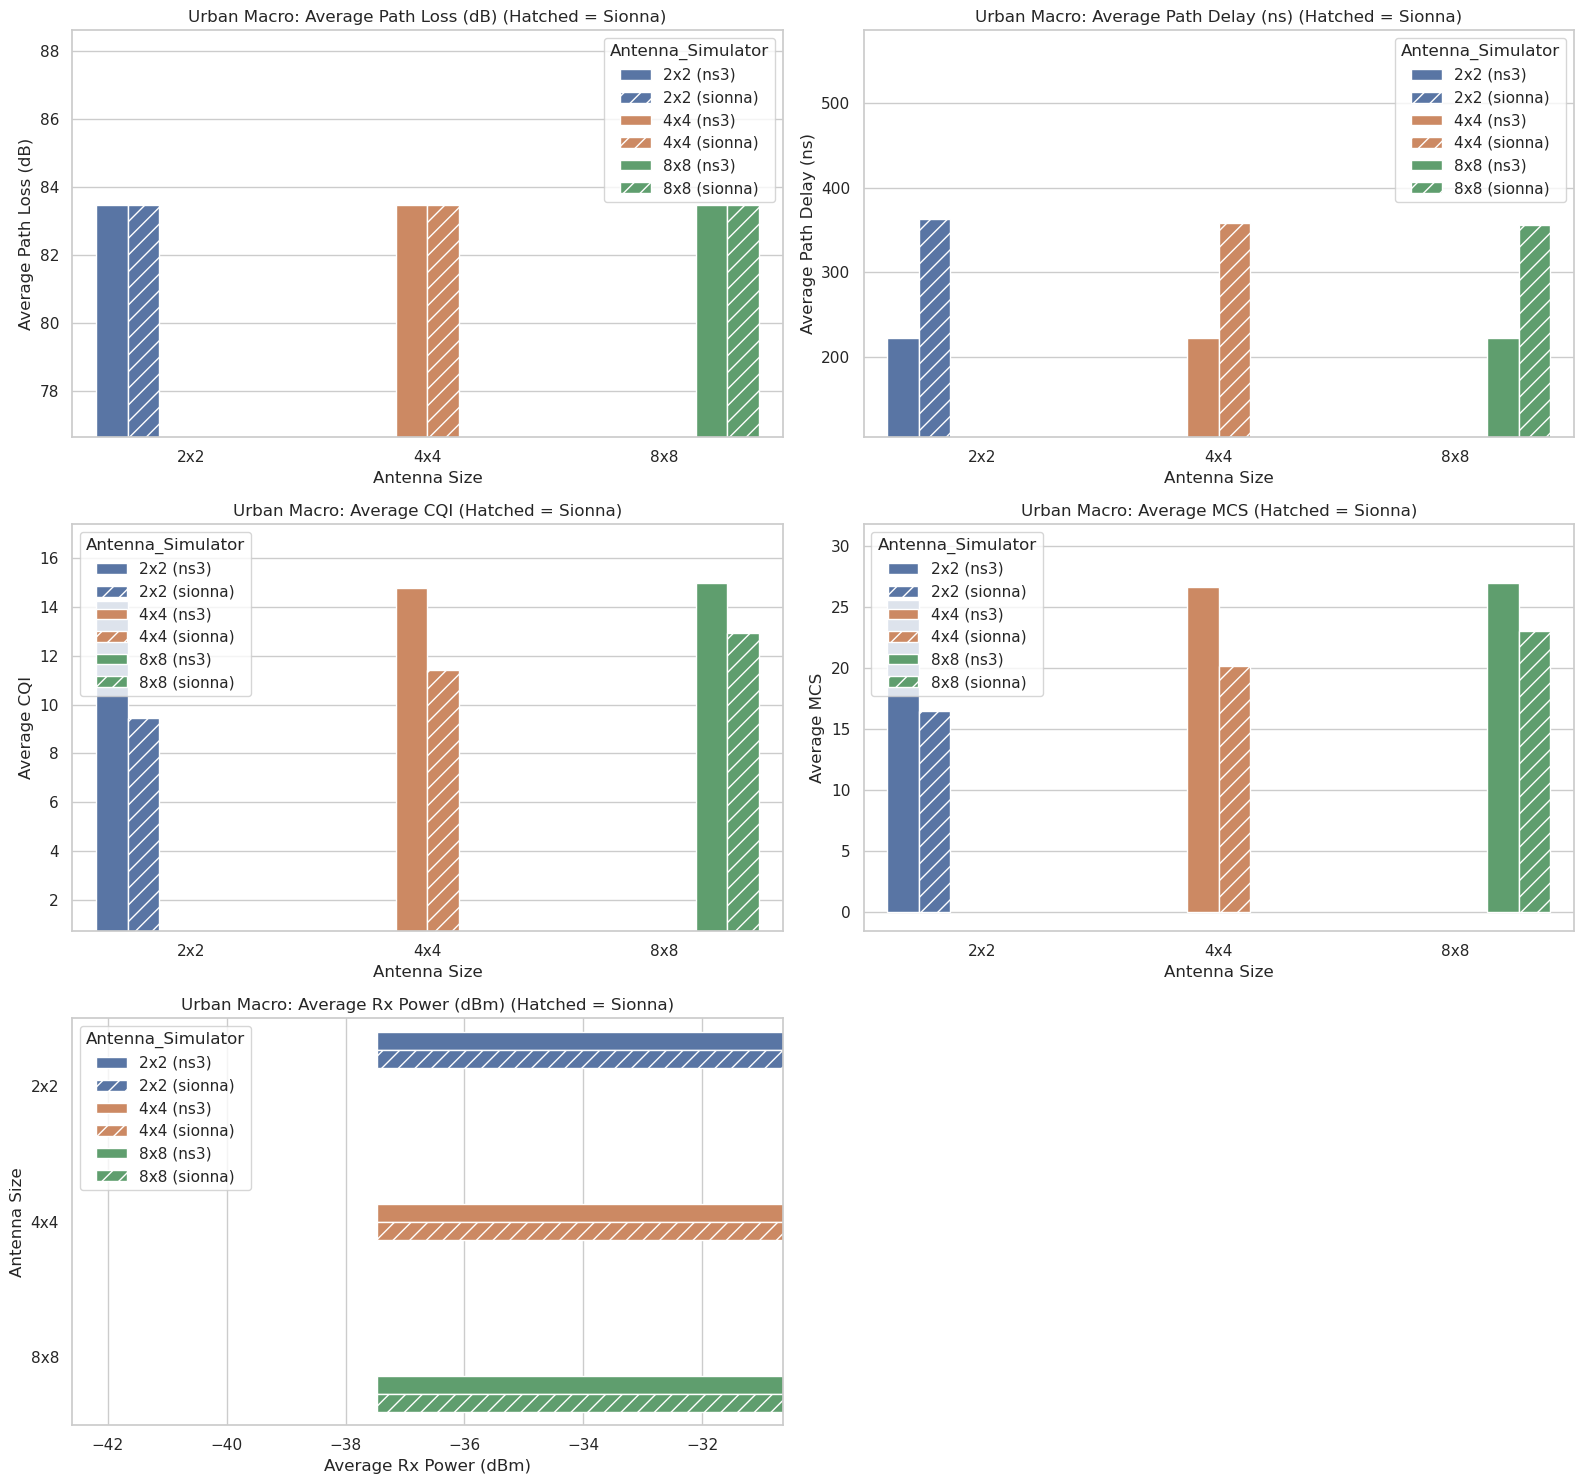
\includegraphics[width=\textwidth]{images/urban_macro_propagation_metrics.png}
    \caption{Urban macro propagation-related metrics by channel mode and gNB array
        size.}
    \label{fig:exp2-urban-macro-propagation}
\end{figure*}


\subsubsection{Energy Consumption-related Metrics}
\label{subsubsec:exp2-urban-macro-energy}\

In Figure \ref{fig:exp2-urban-macro-energy}, the energy consumptions of gNB and UEs by array size, and traffic load are presented.
The power consumption of gNB scales accordingly with both antenna array size and traffic load and both simulators show similar scaling trends.
For instance, both ns-3 and Sionna RT reports approximately $25$ W, $40$ W and $100$ W for $2\times2, 4\times4, 8\times8$ array configurations under low traffic load.
However, Sionna RT reports slightly higher power consumption than ns-3 for all antenna configurations.
The reason is link to lower CQI and MCS values estimated by Sionna RT, which alters resource block allocations and transmission durations compared to ns-3.
These results show that increasing gNB array size improve performance but at the cost of significantly higher energy consumption.

The power consumption of UE remains relatively stable for all antenna configurations in both simulators but scale noticeably with traffic load.
The UE power consumption increases from approximately $0.058$ W at low load to nearly $0.095$ W at high load.
Both simulator observe nearly identical UE power consumption across all configurations but Sionna RT consumes slightly higher energy than ns-3.
This is because UE are constrained to $2 \times 2$ antenna configuration in this experiment.

\begin{figure*}[t]
    \centering
    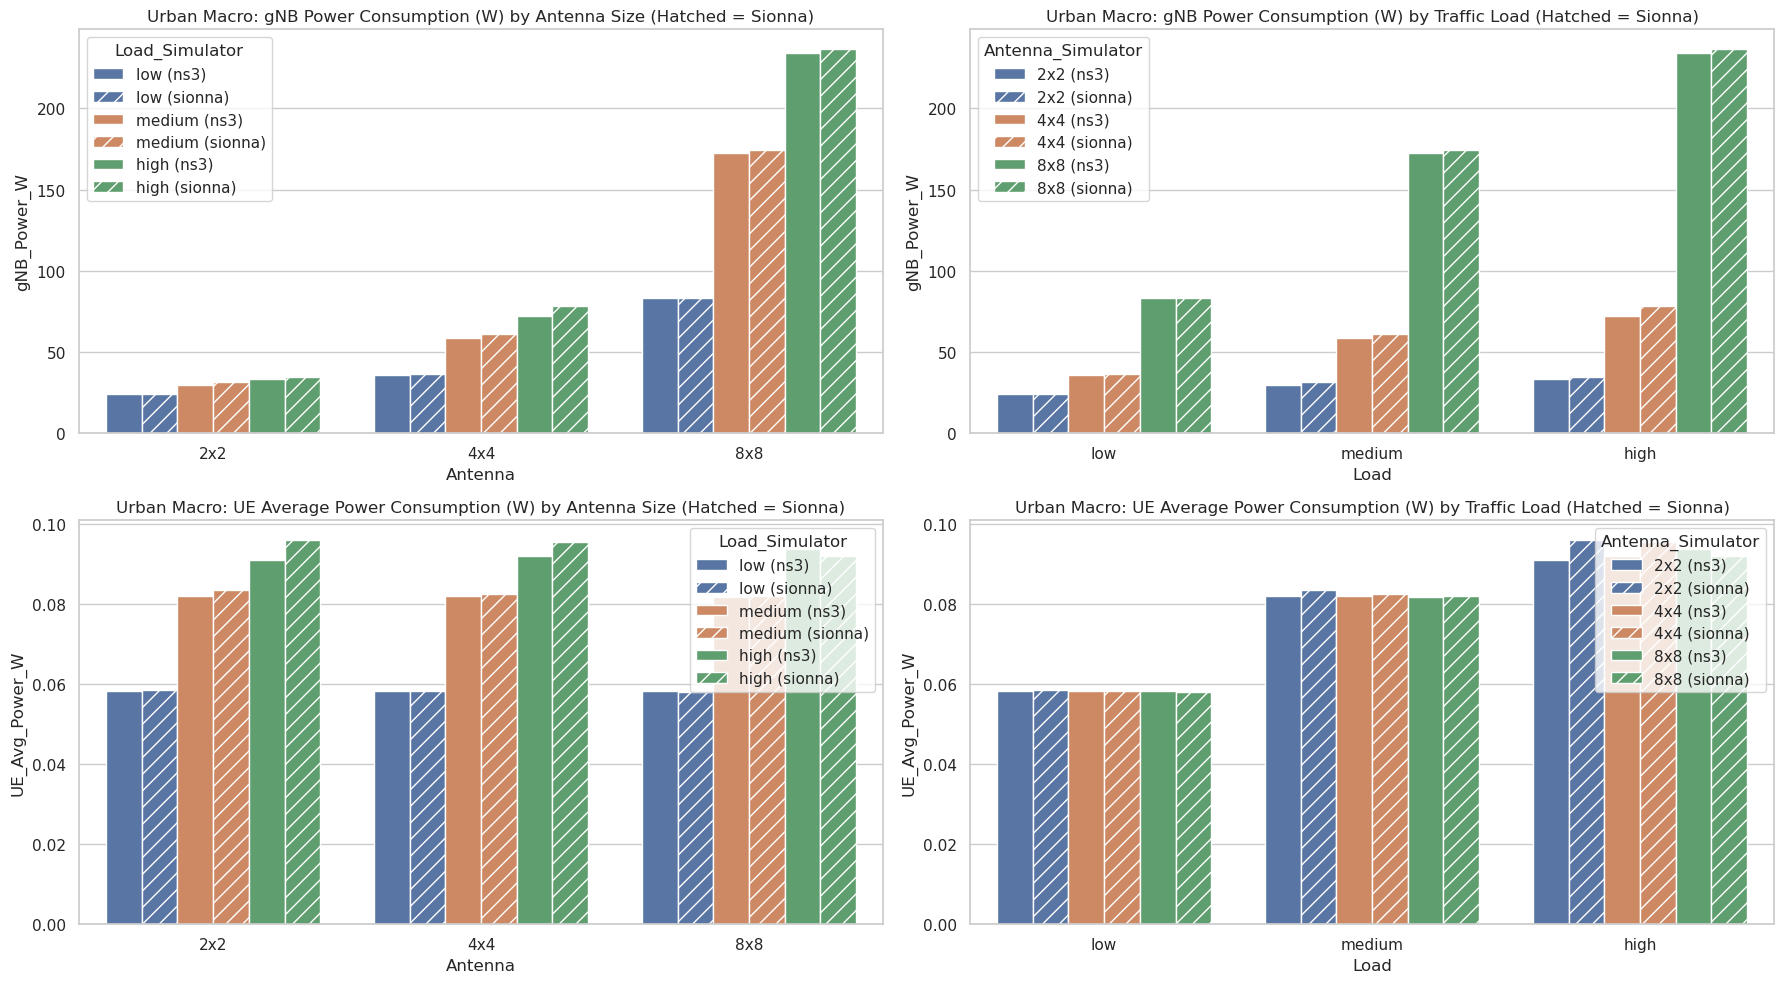
\includegraphics[width=\textwidth]{images/urban_macro_power_consumption.png}
    \caption{Urban macro energy consumptions of gNB and UEs by array size, and
        traffic load.}
    \label{fig:exp2-urban-macro-energy}
\end{figure*}